\chapter{Comparison of MOR Methods} \label{analysis}
The previously mentioned methods for model order reduction will be compared regarding time domain error, frequency domain error and computational speed.
The time domain error will be obtained by comparing the FEM solution to a given approximation.
To get insights into the frequency domain error, the error system of a reduced order model will be analysed.
The computational speed will be determined by measuring the time it takes to generate a ROM.
Here it is assumed that the implementations provided by MORLAB are programmed in a sufficiently effective manner.
For testing the following parameters are used
\begin{gather}
\alpha = 0.1, \quad T = 1, \quad L = 1 \\
n = 100, \quad n_t = 10^{4}
\end{gather}
.

These values are chosen such that it yields results in a timely manner.
Especially \(n_t\) and \(\alpha\) are important for stability of euler scheme.
If both are too low, the euler scheme becomes unstable.
Choosing \(n_t\) too high the time and memory consumption becomes rather large.
There was no exact method for determining the parameters in this way.

\section{Time Domain Error}
The time domain error will defined as \(\epsilon = Y - \hat{Y}\) where \(Y\) and \(\hat{Y}\) denote the matrices storing the output of the systems \(G\) and \(G_r\).
Since the output matrices are usually rather large, it is impractical to use \(\epsilon\) directly.
Therefore  \(||\epsilon||_{F}\) will be considered.
The error is measured using the Frobenius norm to get a measure of the error that respects all data points.
Here two aspects are interesting.
There will be two different initial conditions considered.
The first one is \(x(0, x) = 1\).
It is chosen in this way to display the workings of the boundary condition.
If there were no boundary conditions, for a constant initial condition the system would never cool down since \(\frac{\partial^2 u}{\partial x^2} = 0\) (\ref{eq-1d-h}) at every point in time.
This only holds if there is no input to the system.
Therefore \(u(t) = 0\), where \(u\) denotes the systems input.
The second initial condition is \(x(0, x) = \sin(\frac{2\pi}{L}x)\) with random input.
The initial condition is sinusoidal since it is easy to approximate.

\subsection{Proper Orthogonal decomposition}
Figure \ref{FIG-ERR-POD} shows the \(L2\) error of the solution obtained by the POD model.
\begin{figure}[H]
\centering
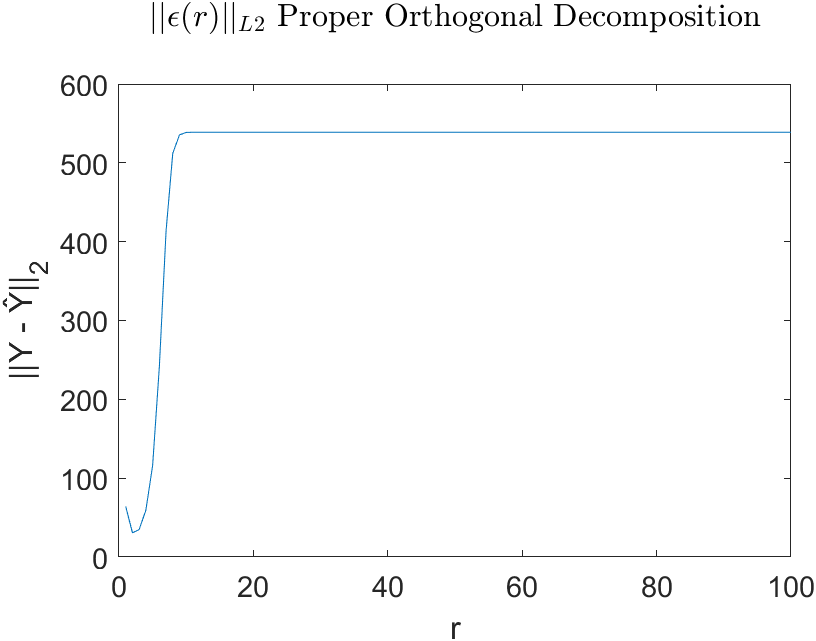
\includegraphics[width=12.5cm]{images/L2_POD}
\caption{L2 Error Proper Orthogonal Decomposition $x(0, x) = 1$}
\label{FIG-ERR-POD}
\end{figure}
It is clearly visible that the error is minimal at  \(r=2\).
This is to be expected since for large \(r\) also low variance modes will be included.
Figure \ref{FIG-POD-VAR} shows that the first two modes capture the most variance with roughly 96\% combined.
It is also visible that all the remaining modes combined only capture 4\%.
\begin{figure}[H]
\centering
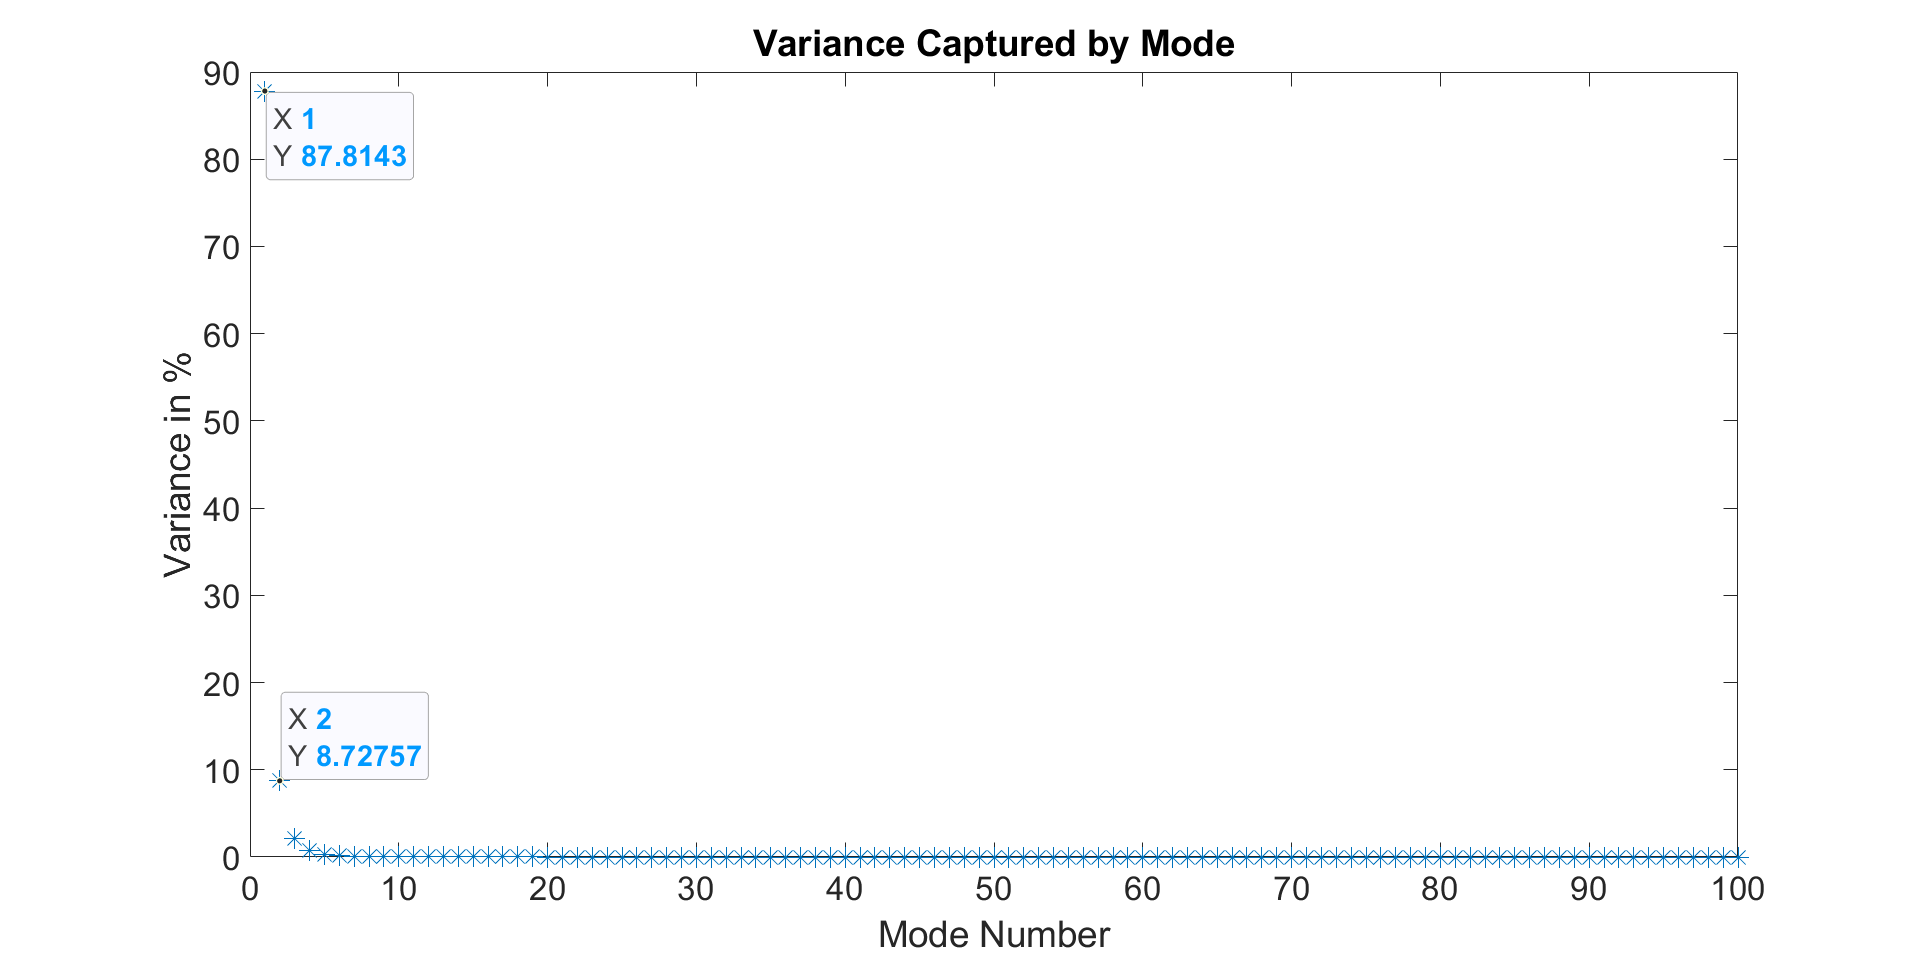
\includegraphics[width=12.5cm]{images/test_modes_pod}
\caption{Variance of POD Modes}
\label{FIG-POD-VAR}
\end{figure}
In this case the low variance modes introduce error, since the initial condition is poorly approximated using orthogonal basis vectors.
This can be seen on figure \ref{fig-pod-100}.
\begin{figure}[H]
\begin{subfigure}[b]{0.5\textwidth}
\centering
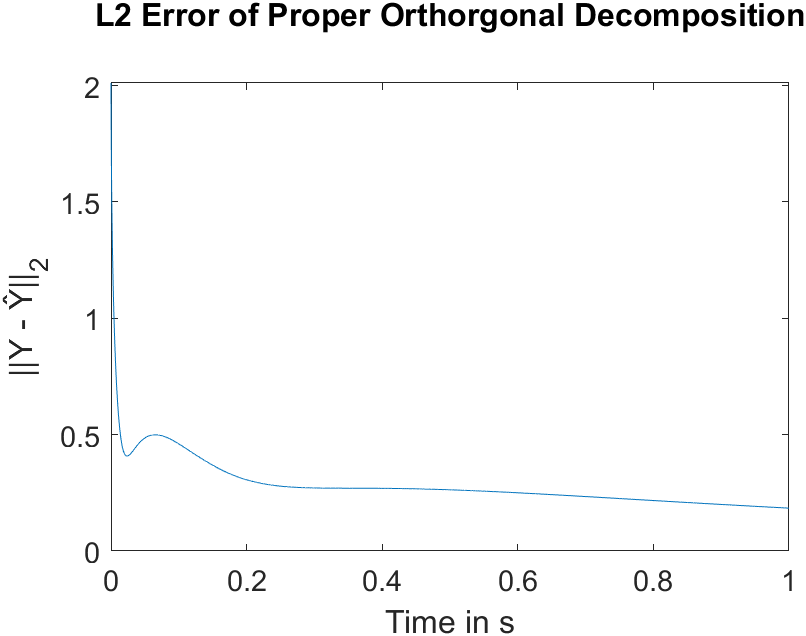
\includegraphics[width=\textwidth]{images/L2_Proper Orthorgonal Decomposition_2_100}
\caption{L2 POD error $r=2$, $n=100$, $x(0, x) = 1$}
\label{fig:fig-pod-2-100}
\end{subfigure}
\begin{subfigure}[b]{0.5\textwidth}
\centering
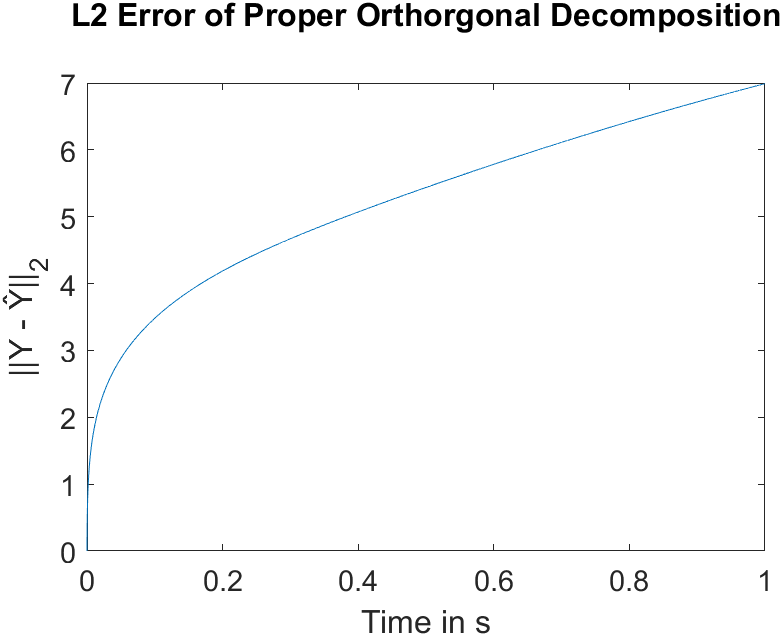
\includegraphics[width=\textwidth]{images/L2_Proper Orthorgonal Decomposition_100_100}
\caption{L2 POD error $r=100$, $n=100$, $x(0, x) = 1$}
\label{fig:fig-pod-100-100}
\end{subfigure}
\label{fig-pod-100}
\end{figure}
The \(L2\) error for \(r=2\) can be seen on figure \ref{fig:fig-pod-2-100}.
Here for \(t=0\) the error is the largest and then drops of quickly and seems to converge to roughly 0.3 whereas the error on figure \ref{fig:fig-pod-100-100} for \(r=100\) is almost zero at \(t=0\) and diverges.
This problem does not only apply to the initial condition, this problem if the snapshot matrix contains vectors that are poorly approximated using orthogonal basis vectors.
The low variance modes do not introduce error. 
In fact they even lower the error and the error is lower in general as it can be seen on figure \ref{FIG-ERR-POD-SIN}.
\begin{figure}[H]
\centering
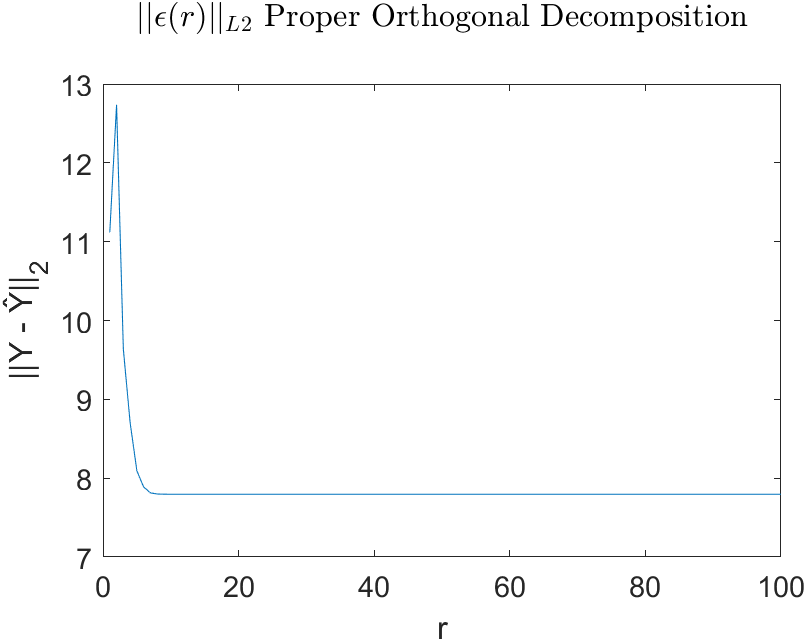
\includegraphics[width=12.5cm]{images/L2_POD_SIN}
\caption{L2 Error Proper Orthogonal Decomposition $x(0, x) = \sin(\frac{2\pi}{L}x)$}
\label{FIG-ERR-POD-SIN}
\end{figure}
Another difference is that for $x(0, x) = \sin(\frac{2\pi}{L}x)$ the error distribution over time does not differ as much for \(r=100\) and \(r=2\).
This can be observed on figure \ref{fig:fig-pod-2-100-sina} and \ref{fig:fig-pod-100-100-sinb}.
\begin{figure}[H]
\begin{subfigure}[b]{0.5\textwidth}
\centering
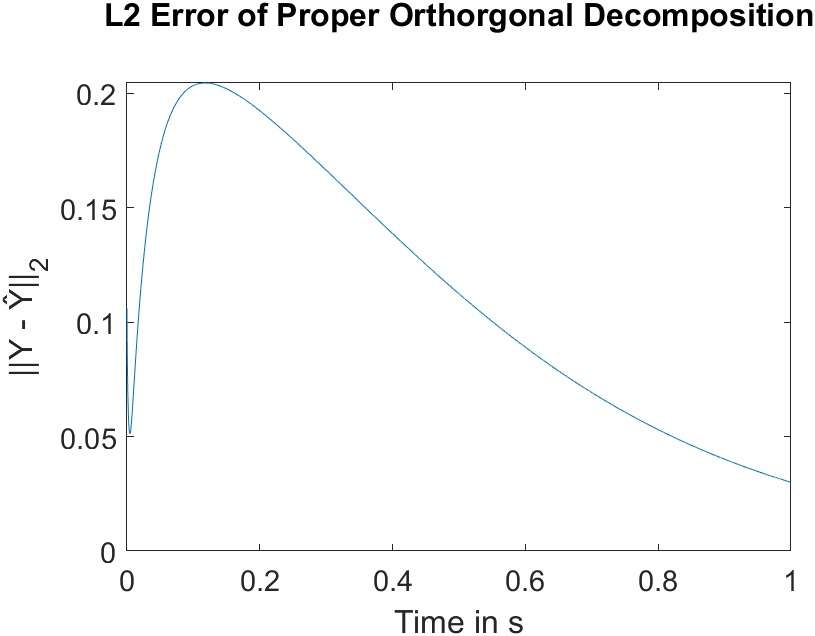
\includegraphics[width=\textwidth]{images/L2_Proper Orthorgonal Decomposition_2_100sin}
\caption{ $r=2$, $n=100$, $x(0, x) = \sin(\frac{2\pi}{L}x)$}
\label{fig:fig-pod-2-100-sina}
\end{subfigure}
\begin{subfigure}[b]{0.5\textwidth}
\centering
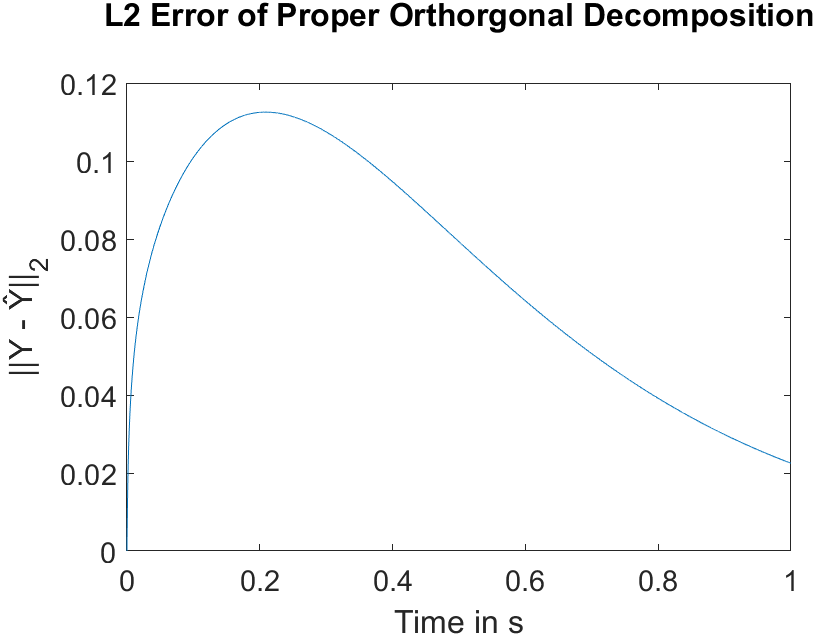
\includegraphics[width=\textwidth]{images/L2_Proper Orthorgonal Decomposition_100_100sin}
\caption{$r=100$, $n=100$, $x(0, x) = \sin(\frac{2\pi}{L}x)$}
\label{fig:fig-pod-100-100-sinb}
\end{subfigure}
\label{fig-pod-100-sin}
\caption{L2 POD error}
\end{figure}


\subsection{Modal Truncation}
Figure \ref{FIG-ERR-MT} shows the \(L2\) error of the ROM obtained by Modal Truncation.
\begin{figure}[H]
\begin{subfigure}[b]{0.5\textwidth}
\centering
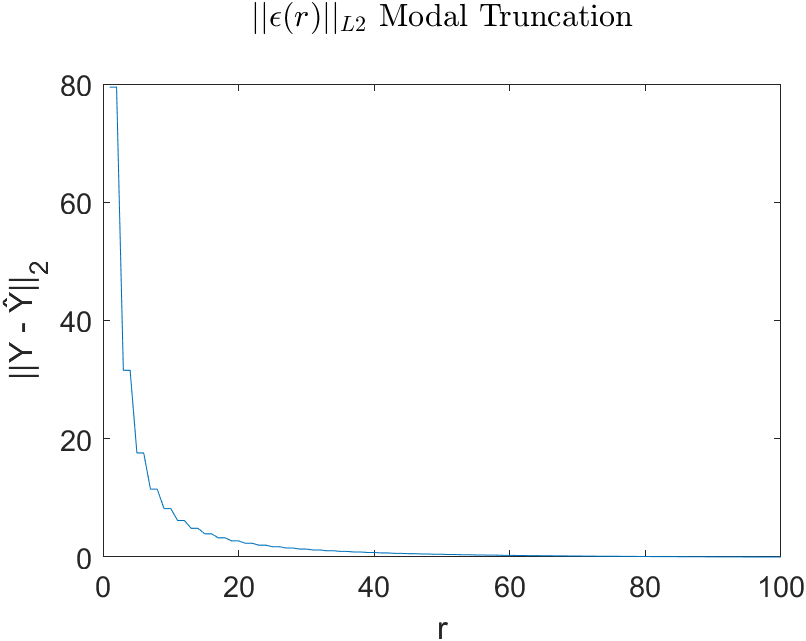
\includegraphics[width=\textwidth]{images/L2_MT}
\caption{$x(0, x) = 1$}
\label{FIG-ERR-MT}
\end{subfigure}
\begin{subfigure}[b]{0.5\textwidth}
\centering
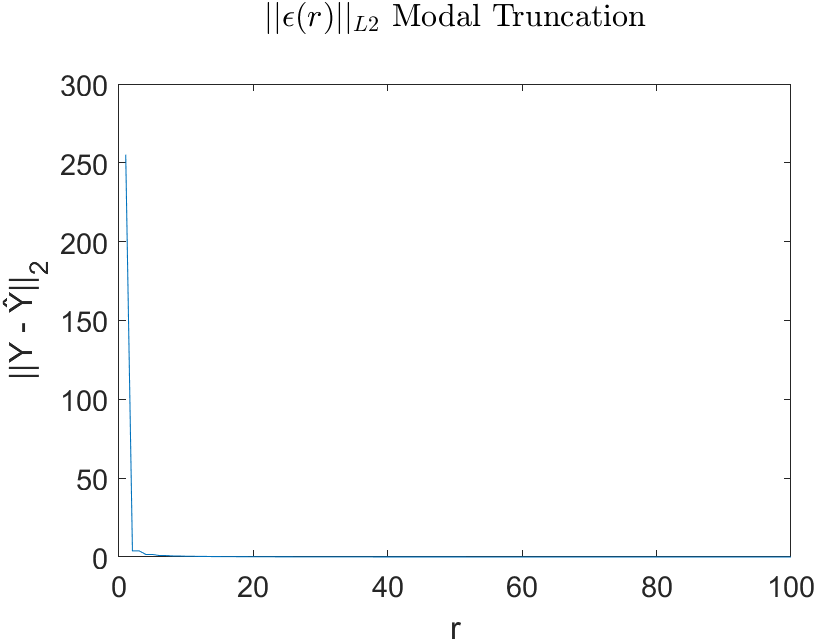
\includegraphics[width=\textwidth]{images/L2_MT_SIN}
\caption{$x(0, x) = \sin(\frac{2\pi}{L}x)$}
\label{FIG-ERR-MT-SIN}
\end{subfigure}
\caption{L2 Error Balanced Truncation}
\end{figure}
It shows that as \(r\) increases the error converges to zero.
This is to be expected since as \(r\) increases \(G_r\) becomes closer to \(G\).
For \(x(0, x) = \sin(\frac{2\pi}{L}x)\) the error starts off significantly higher but decays even faster as it can be seen on figure \ref{FIG-ERR-MT-SIN}.
\newpage
\subsection{Balanced Truncation}
Figure \ref{FIG-ERR-BT} shows the \(L2\) error of the ROM obtained by Balanced Truncation.
\begin{figure}[H]
\begin{subfigure}[b]{0.5\textwidth}
\centering
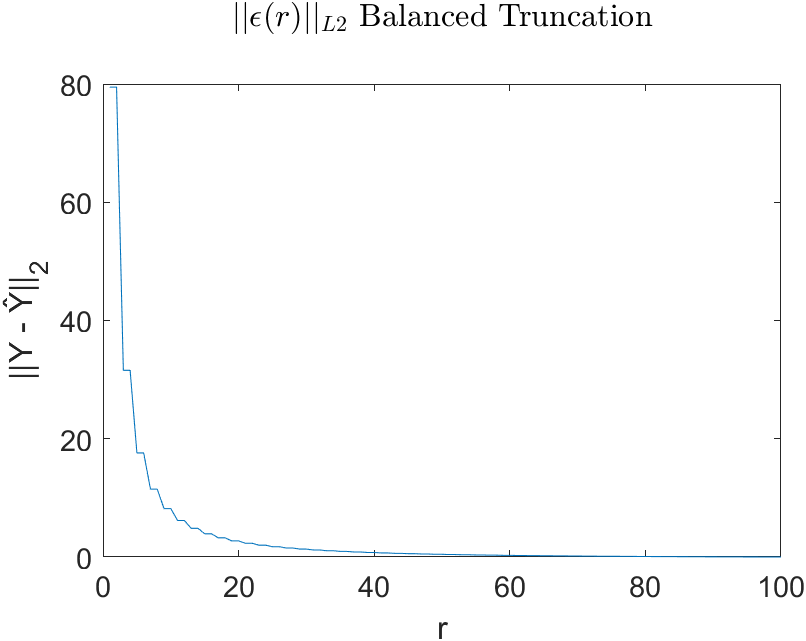
\includegraphics[width=\textwidth]{images/L2_BT}
\caption{$x(0, x) = 1$}
\label{FIG-ERR-BT}
\end{subfigure}
\begin{subfigure}[b]{0.5\textwidth}
\centering
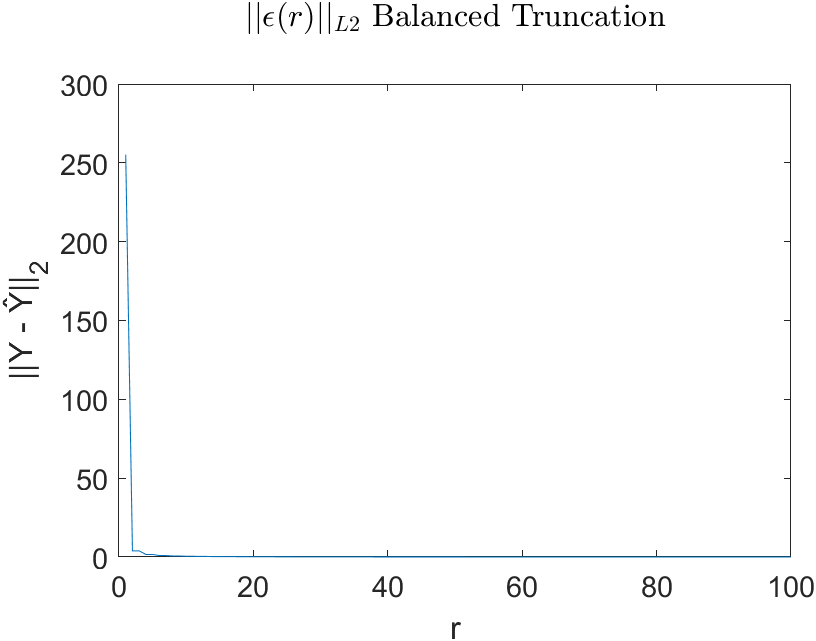
\includegraphics[width=\textwidth]{images/L2_BT_SIN}
\caption{$x(0, x) = \sin(\frac{2\pi}{L}x)$}
\label{FIG-ERR-BT-SIN}
\end{subfigure}
\caption{L2 Error Balanced Truncation}
\end{figure}
It shows that as \(r\) increases the error converges to zero.
This is to be expected since as \(r\) increases \(G_r\) becomes closer to \(G\).
As expected the results for Modal Truncation and Balanced Truncation are the same.

\subsection{Hankel Norm Approximation}
Figure \ref{FIG-ERR-HNA} shows the \(l2\) error of the output generated by the HNA model.
Here it is striking that for \(r > 34\) the model does not generate usable output.
This is due to the reason that for the chosen settings the used euler scheme does not converge for \(r > 34\).
Decreasing \(\Delta t\) yields results for \(r > 34\) but it becomes prohibitively expensive to compute.
However for \(r \leq \frac{n}{3}\) the error converges to zero as \(r\) increases.

\begin{figure}[H]
\begin{subfigure}[b]{0.5\textwidth}
\centering
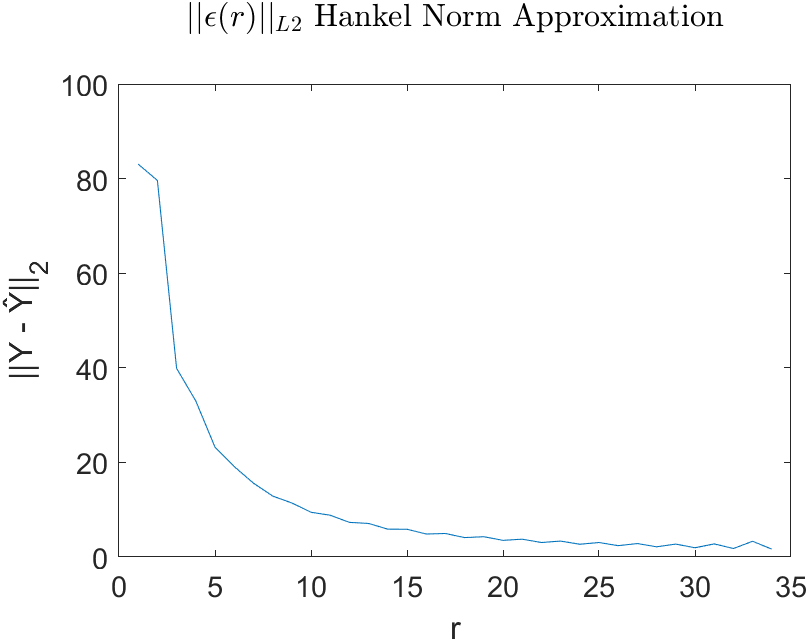
\includegraphics[width=\textwidth]{images/L2_HNA}
\caption{$x(0, x) = 1$}
\label{FIG-ERR-HNA}
\end{subfigure}
\begin{subfigure}[b]{0.5\textwidth}
\centering
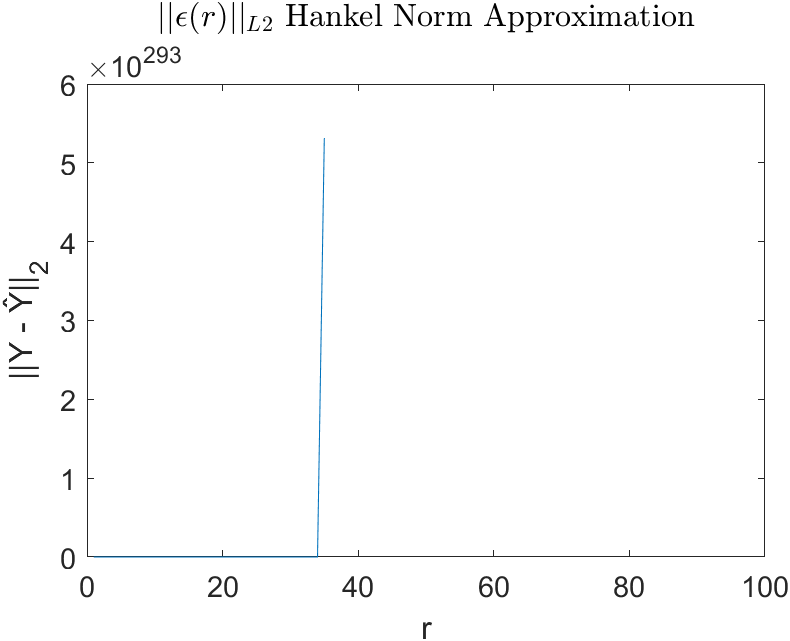
\includegraphics[width=\textwidth]{images/L2_HNA_SIN}
\caption{$x(0, x) = \sin(\frac{2\pi}{L}x)$}
\label{FIG-ERR-HNA-SIN}
\end{subfigure}
\caption{\(L2\) Error Hankel Norm Approximation}
\end{figure}
It is noticeable that similar to BT and MT the error for \(x(0, x) = \sin(\frac{2\pi}{L}x)\) starts higher than for \(x(0, x) = 1\) and then decays quite fast.

\subsection{Comparison of Time Domain Error}
Figure \ref{FIG-BOX-L2} shows the measured \(L2\) error plotted as a box plot to compare them. 
Since the range of the data is too large to plot it in this way, the data is transformed using \(\log_{10}\).
This results in the problem that zeros cannot be expressed.
It is the case for Modal Truncation at \(r = 100\).
\begin{figure}[H]
\begin{subfigure}[b]{0.5\textwidth}
\centering
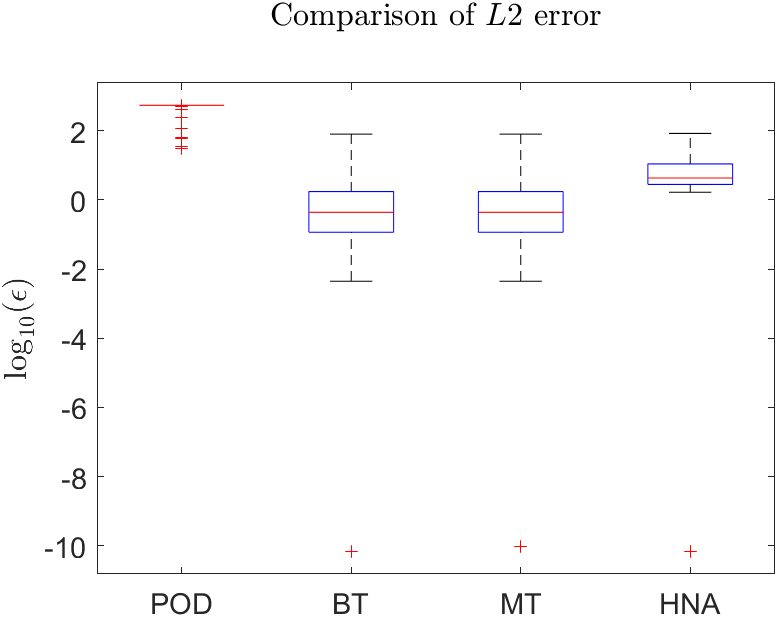
\includegraphics[width=\textwidth]{images/L2_BOX}
\caption{$x(0, x) = 1$}
\label{FIG-BOX}
\end{subfigure}
\begin{subfigure}[b]{0.5\textwidth}
\centering
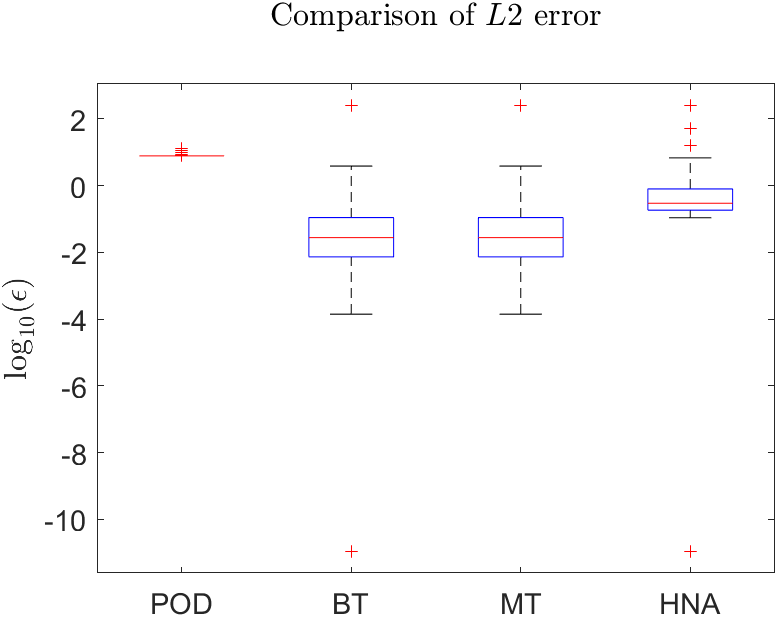
\includegraphics[width=\textwidth]{images/L2_BOX_SIN}
\caption{$x(0, x) = \sin(\frac{2\pi}{L}x)$}
\label{FIG-BOX-SIN}
\end{subfigure}
\caption{Box Plot of \(L2\) Error}
\label{FIG-BOX-L2}
\end{figure}
It is noticeable that the relative difference between each of the methods stays roughly the same for both initial conditions.
As expected the error of all methods is higher in general for \(x(0, t) = 1\).
The box for POD is the one with the lowest IQR while having the largest \(\log\) error, meaning that the error of POD converges the fastest but also it does not converge to zero.
Keep in mind that the seemingly large IQR of the error of MT and BT is actually small, because the \(\log\) error is depicted.
Therefore the error of MT and BT converge faster than the one of HNA while the error is smaller in general.
Therefore BT and MT are the best choices when considering \(L2\) time domain error.



\section{Frequency Domain Error}
The frequency domain error for \(G_{\epsilon }= G - G_r\) will be determined using the \(H_{\infty}\) norm.
For a MIMO system this is the maximum singular value of the frequency response of the transfermatrix.
It can be interpreted as the maximum gain from the \(i^{th}\) input to the \(i^{th}\) output \cite{eugenio}.
The \(H2\) cannot be used to get a measure of the error since the ROM that HNA yields has nonzero feedthrough matrix, therefore \(||G_{\epsilon}||_{H_{2}}\) is infinite. 

\subsection{Proper Orthogonal Decomposition}
Since the ROM obtained by POD is derived from a solution of the full state system, it is depended on the initial condition.
Therefore the frequency domain error is also dependent on the initial condition.
This can be seen on figure \ref{FIG-H-POD} and figure \ref{FIG-H-POD-SIN}, they clearly differ from each other.
For \(x(0, x) = 1\) there are two distinct spikes at \(r=49\) and \(r=63\).
The reason for them is unclear, however the larger one is three orders of magnitude higher than the peak in the \(H_{\infty}\) error for $x(0, x) =  \sin(\frac{2\pi}{L}x)$.
This peak is not depicted on figure \ref{FIG-H-POD-SIN} since it is one single data point that is 14 orders of magnitude higher than the remaining data points.
The peaks on figure \ref{FIG-H-POD} are not removed since the remaining data points are also large.
\begin{figure}[H]
\begin{subfigure}[b]{0.5\textwidth}
\centering
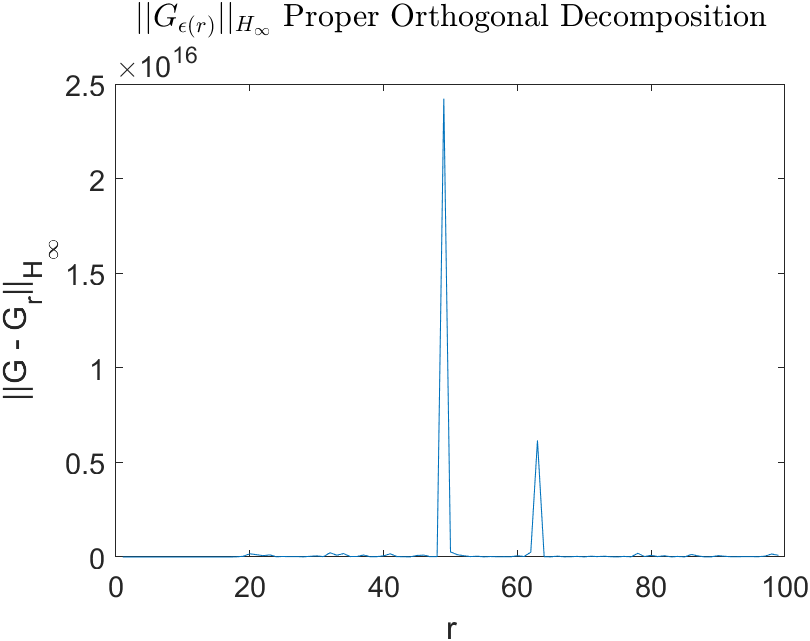
\includegraphics[width=\textwidth]{images/freq/H_POD}
\caption{$H_{\infty}$ error of POD, $x(0, x) = 1$}
\label{FIG-H-POD}
\end{subfigure}
\begin{subfigure}[b]{0.5\textwidth}
\centering
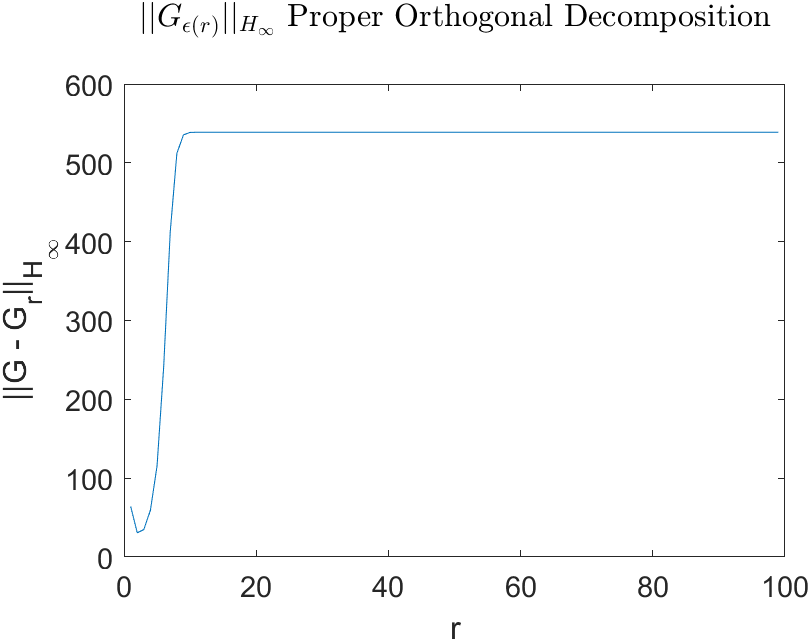
\includegraphics[width=\textwidth]{images/freq/H_POD_SIN}
\caption{$H_{\infty}$ error of POD, $x(0, x) =  \sin(\frac{2\pi}{L}x)$}
\label{FIG-H-POD-SIN}
\end{subfigure}
\caption{$H_{\infty}$ error of POD}
\label{FIG-H-POD-1}
\end{figure}
In general the error in frequency domain is larger for \(x(0, x) = 1\) than for \(x(0, x) =  \sin(\frac{2\pi}{L}x)\). 
This matches the behaviour of the time domain error.

\subsection{Modal Truncation and Balanced Truncation}
The frequency domain error of Modal Truncation and Balanced Truncation is independent of the initial condition.
For small \(r\) it is comparably large and converges towards zero as \(r\) gets larger.
As expected the results of Balanced Truncation and Modal Truncation is the same as figure \ref{FIG-H-BTMT} shows.
\begin{figure}[H]
\begin{subfigure}[b]{0.5\textwidth}
\centering
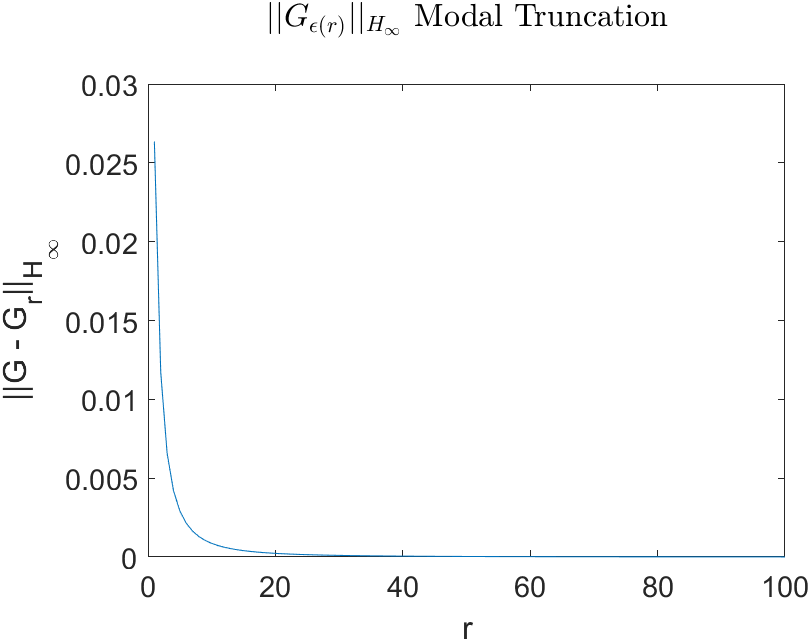
\includegraphics[width=\textwidth]{images/freq/H_MT}
\caption{$H_{\infty}$ error of Modal Truncation}
\label{FIG-H-MT}
\end{subfigure}
\begin{subfigure}[b]{0.5\textwidth}
\centering
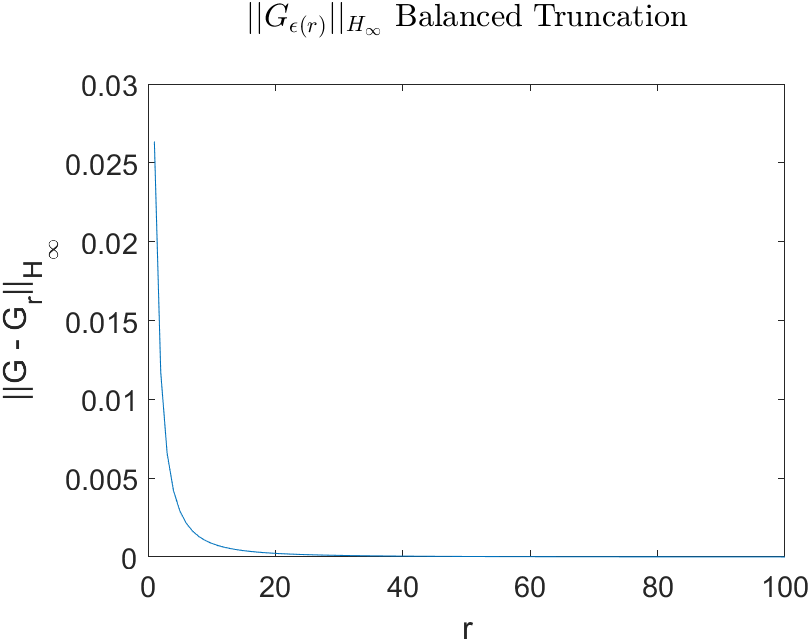
\includegraphics[width=\textwidth]{images/freq/H_BT}
\caption{$H_{\infty}$ error of Balanced Truncation}
\label{FIG-H-BT}
\end{subfigure}
\caption{$H_{\infty}$ error of Balanced Truncation and Modal Truncation}
\label{FIG-H-BTMT}
\end{figure}


\subsection{Hankel Norm Approximation}
Figure \ref{FIG-H-HNA} shows the frequency domain error of HNA.
Similar to BT and MT the error is large for small \(r\) and decays as \(r\) gets larger.
However the error overall is smaller than for BT and HNA.
\begin{figure}[H]
\centering
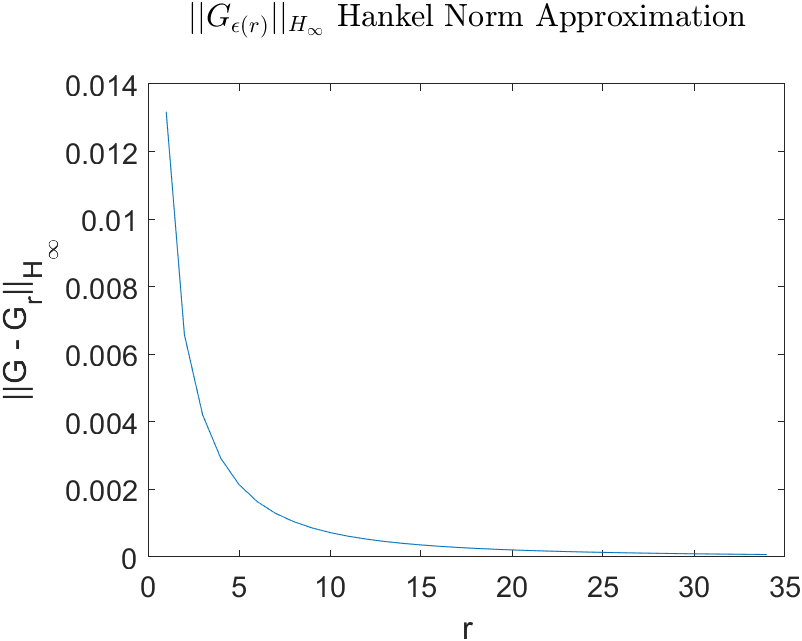
\includegraphics[width=0.5\textwidth]{images/freq/H_HNA}
\caption{$H_{\infty}$ error of Hankel Norm Approximation}
\label{FIG-H-HNA}
\end{figure}

\subsection{Comparison of Time Domain Error}
To compare the results directly, the error of the ROMs for all \(r\) are plotted using a box plot.
However the error is not directly used because of some large peaks in the data, which would render the plot unreadable.
Instead the \(\log_{10}\) of each data point is taken.
This is possible since all data points are strictly positive, therefore the order of the data points is preserved while lowering the range between outliers.
The box plot can be seen on figure \ref{FIG-H-BOX}.
\begin{figure}[H]
\centering
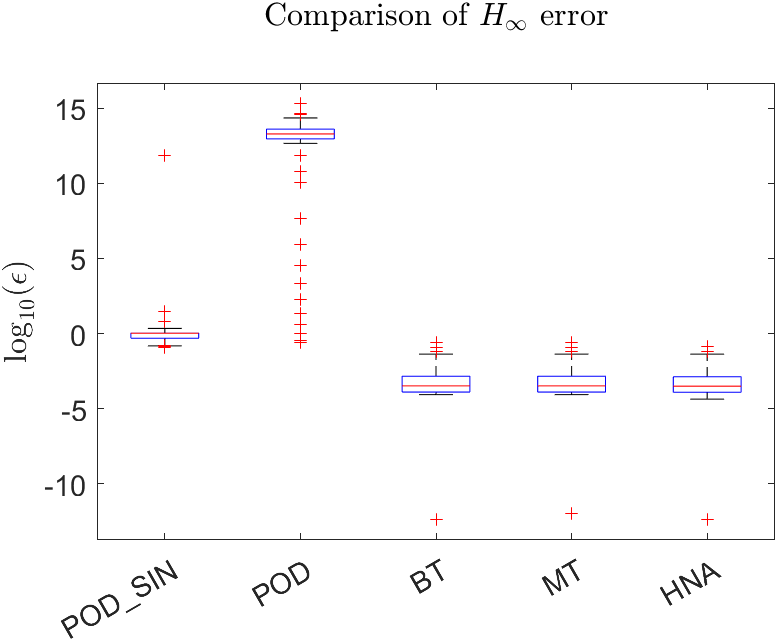
\includegraphics[width=0.5\textwidth]{images/freq/H_BOX}
\caption{Box Plot of $H_{\infty}$ error}
\label{FIG-H-BOX}
\end{figure}
Where 'POD' denotes the POD ROM for \(x(0, x) = 1\) and 'POD\_SIN' denotes the POD ROM for \(x(0, x) =  \sin(\frac{2\pi}{L}x)\).
The plot shows that the frequency domain error of the ROM obtained using POD with \(x(0, x) = 1\) yields by far the worst results.
The best choice for minimal \(H_{\infty}\) error here is clearly HNA. 
The error of HNA is significantly lower than the error of the other three methods.

\section{Processing Time}
The processing time is obtained by measuring the time it takes to build the reduced order model.
To make sure that the measurements are reliable to some degree, each measurement is taken ten times.
This choice is arbitrary, but was taken to keep overall computing time in check.
Those measurements are depicted as box plots in the following figures.

\subsection{Proper Orthogonal Decomposition}
Figure \ref{FIG-T-POD} shows the processing time of POD.
It can be observed that the time it takes to compute a POD model, is quite constant for  \(1 \geq r \geq 100\).
This implies that the implementation of the algorithm is efficient to an extend that the range of \(r\) is too small to gain information about the relation between \(r\) and the processing time.
The measurements are mainly between 0.012 and 0.022 seconds.
\begin{figure}[H]
\centering
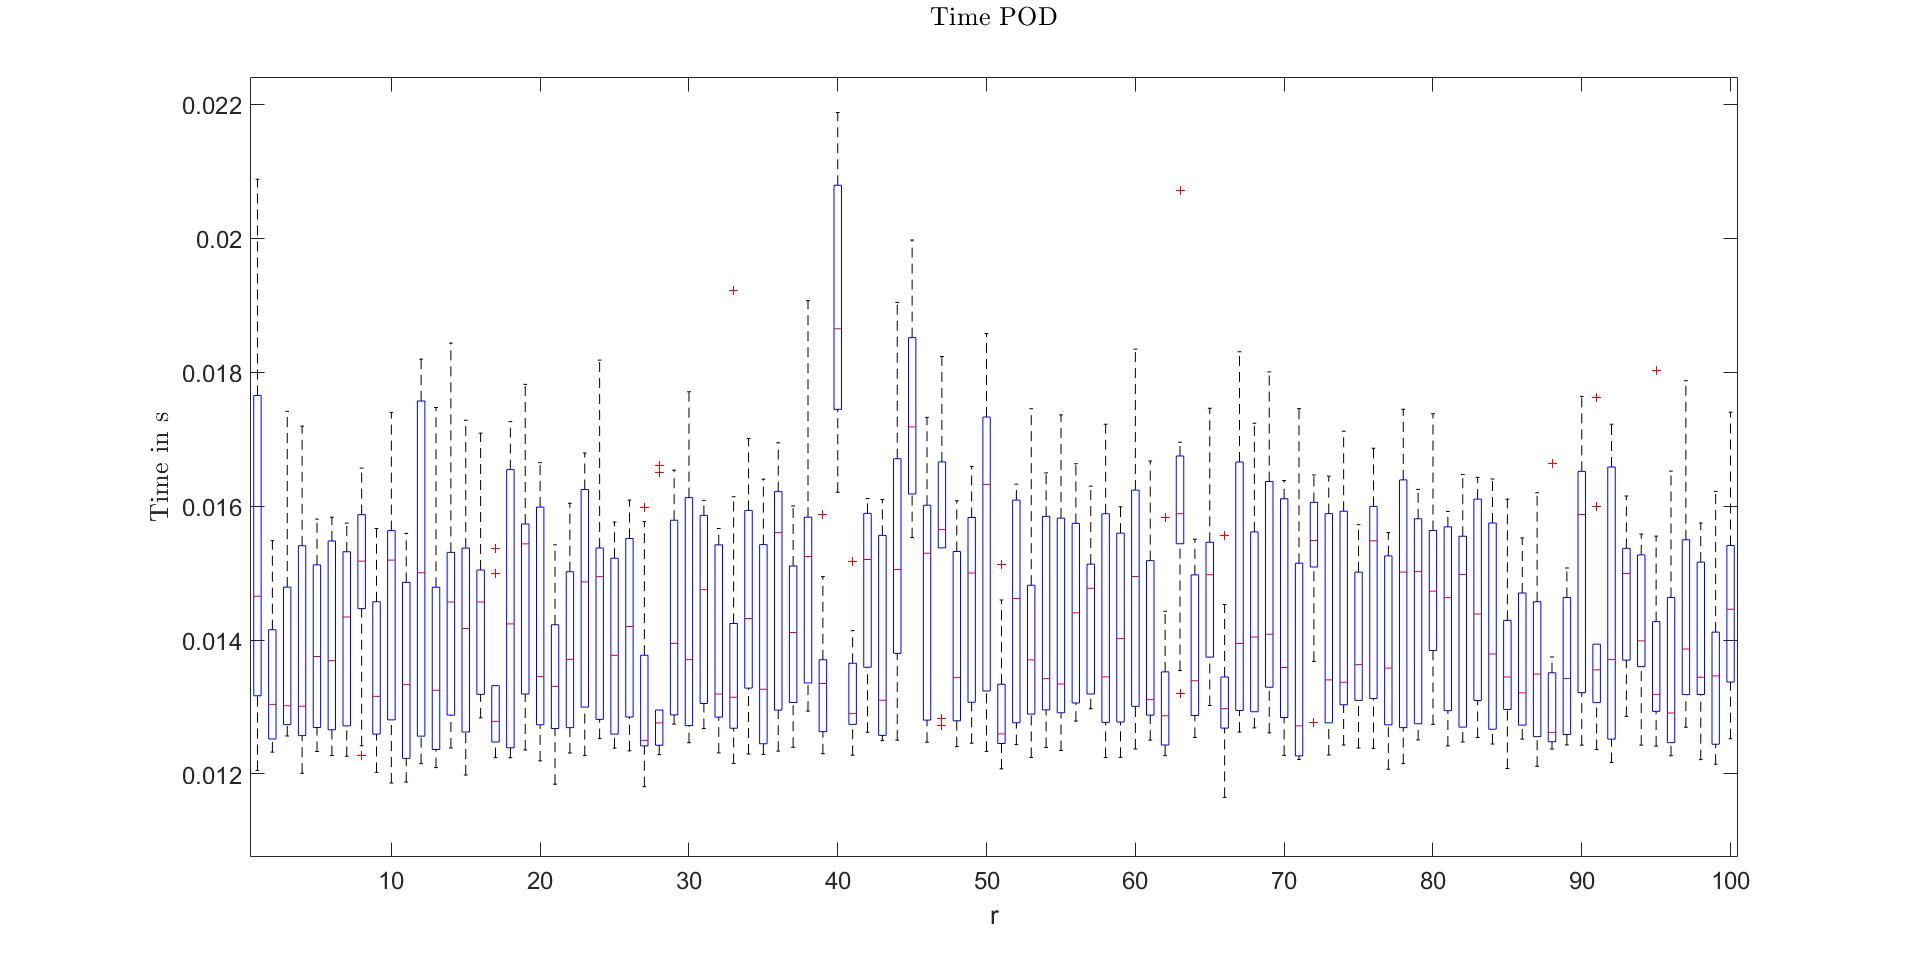
\includegraphics[width=\textwidth]{images/time/POD}
\caption{Processing time POD}
\label{FIG-T-POD}
\end{figure}



\subsection{Modal Truncation}
Figure \ref{FIG-T-MT} shows the processing time of modal truncation.
It is noticeable that \(r = 100\) yields the lowest time to compute.
This is to be expected since in this case modal truncation is equal to applying a coordinate transform to the original system.
For \(r \neq 100\) there is seemingly some \(r\) around fifty that offers some optimal computing speed.
Again this could be due to the rather small range of  \(r\).
The most measurements are in a range between 3.5 and 5 milliseconds.
\begin{figure}[H]
\centering
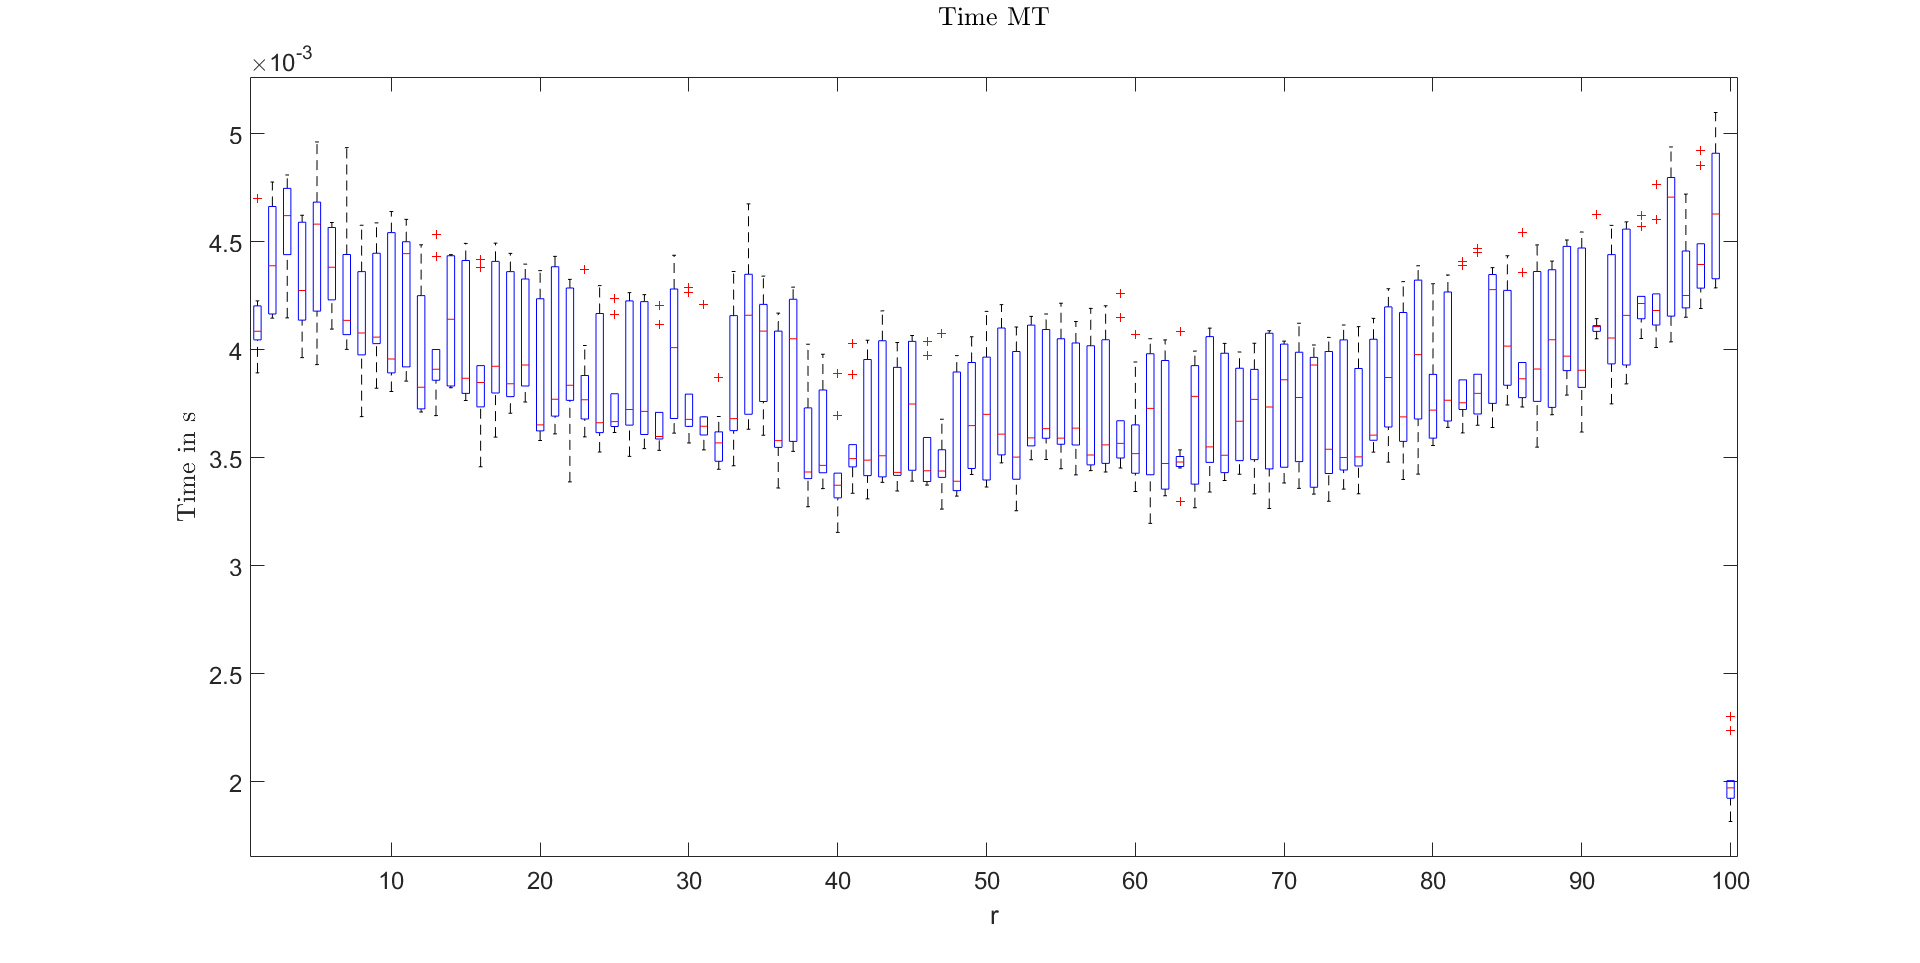
\includegraphics[width=\textwidth]{images/time/MT}
\caption{Processing time MT}
\label{FIG-T-MT}
\end{figure}


\subsection{Balanced Truncation}
Figure \ref{FIG-T-BT} displays the processing time with respect to the model order \(r\).
Again it is fairly constant where the majority of measurements is in a range between 0.03 and 0.04 seconds.
\begin{figure}[H]
\centering
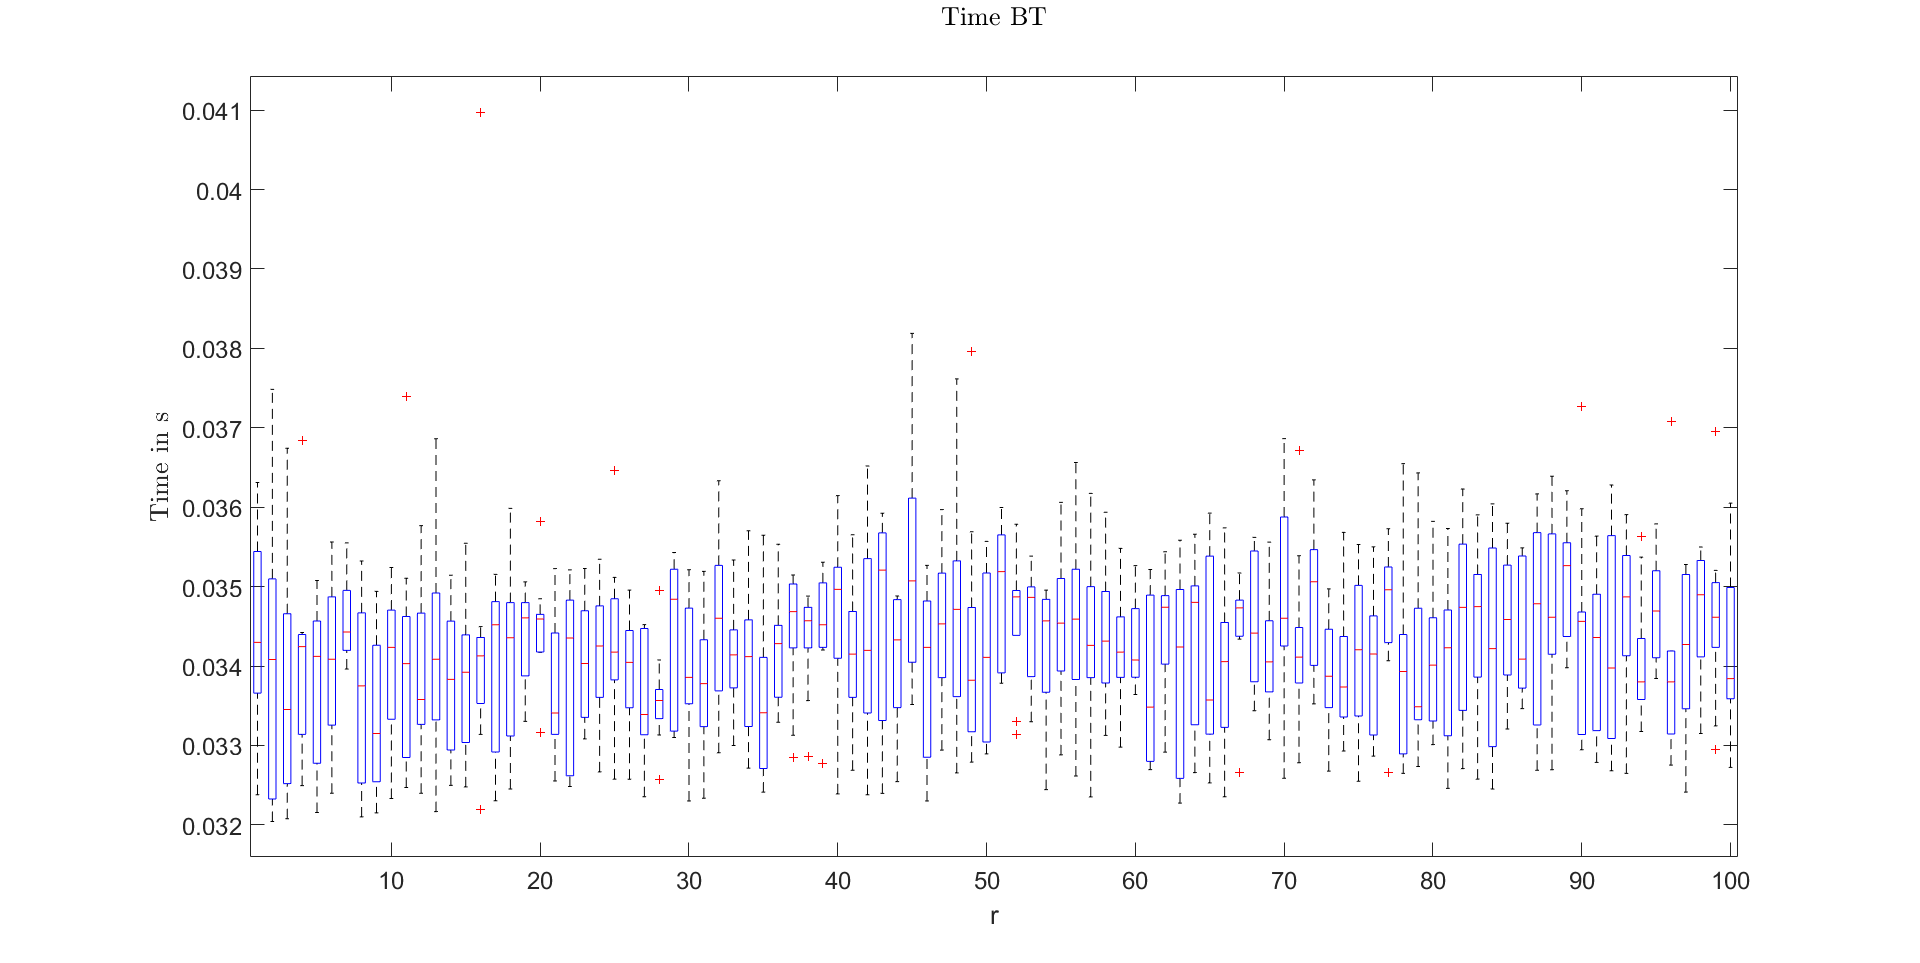
\includegraphics[width=\textwidth]{images/time/BT}
\caption{Processing time BT}
\label{FIG-T-BT}
\end{figure}


\subsection{Hankel Norm Approximation}
Figure \ref{FIG-T-HNA} shows the the processing time dependent on the model order.
It is striking that for \(r = 99\) and \(r = 100\) the processing time is significantly lower than in the remaining measurements.
The exact reason for this is unclear, however it could be speculated that for \(r=100\) only a balanced realization is computed and therefore many steps of the algorithm could be skipped.
Except for those two outliers the range of the majority of the measurements is 0.036 to 0.043 seconds.
\begin{figure}[H]
\centering
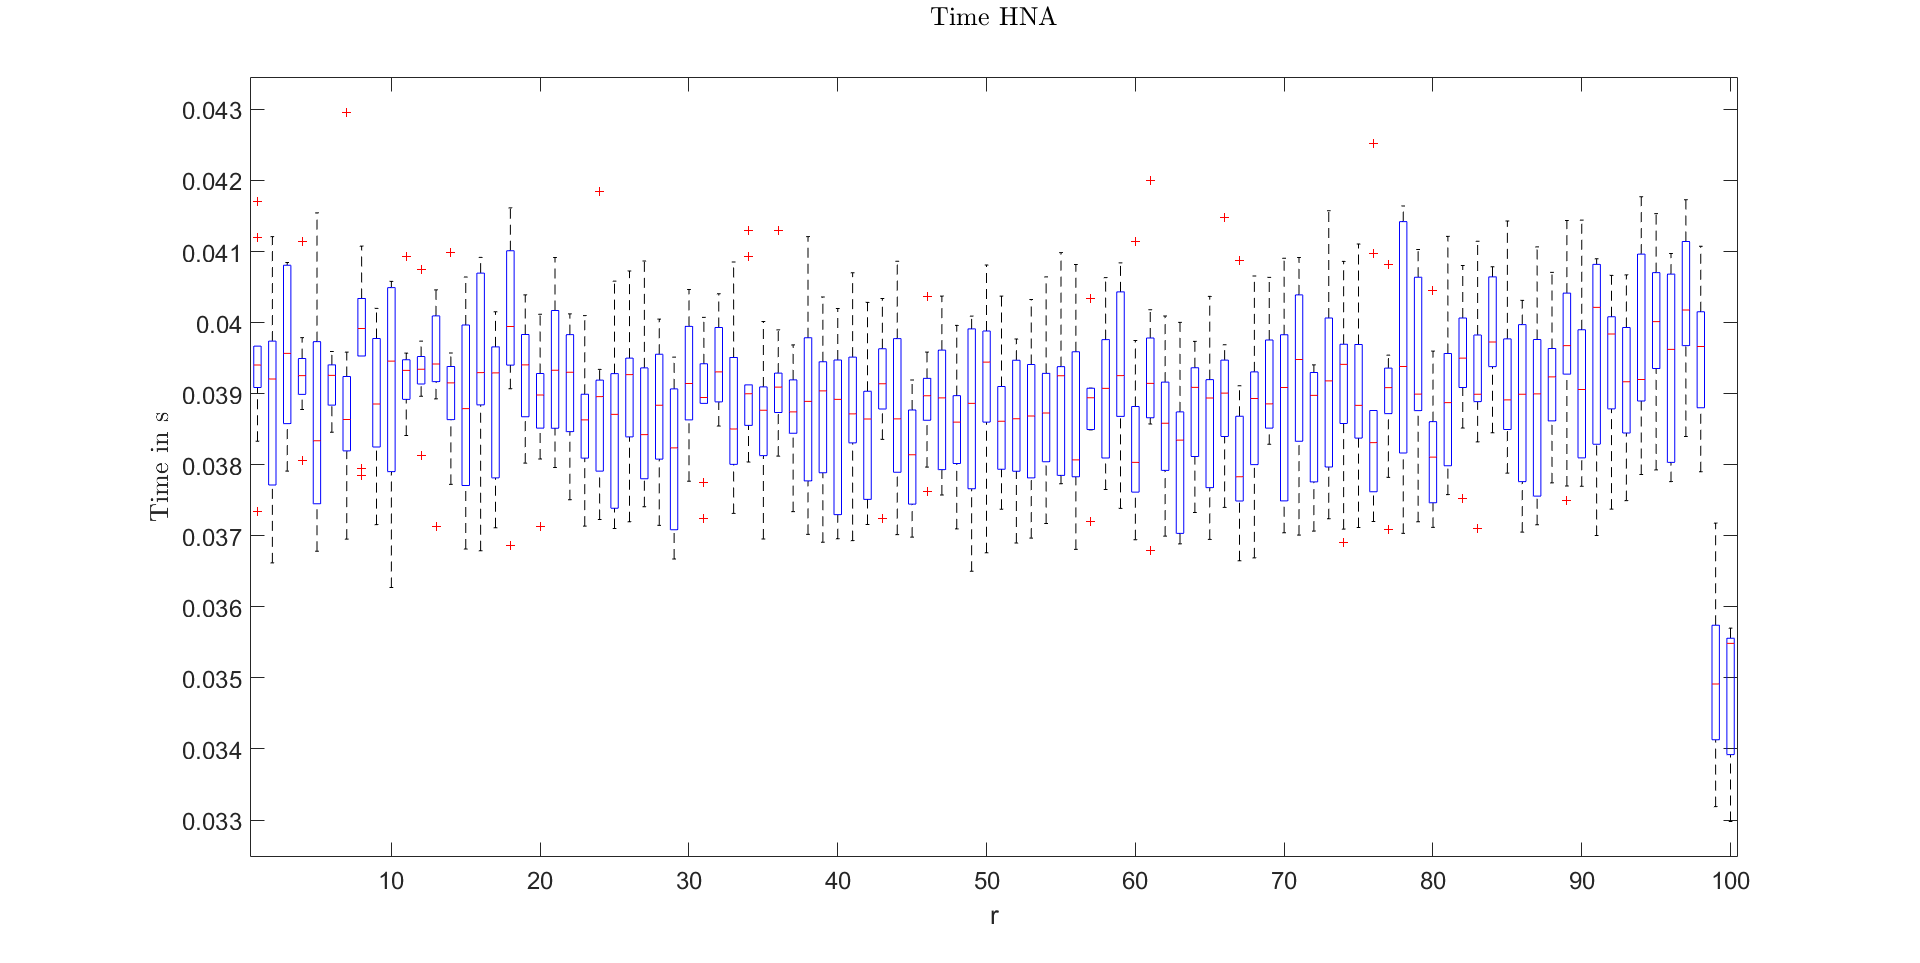
\includegraphics[width=\textwidth]{images/time/HNA}
\caption{Processing time HNA}
\label{FIG-T-HNA}
\end{figure}

\subsection{Comparison of processing time}
The fastest method here is modal truncation.
It is roughly one order of magnitude faster than the remaining methods.
Balanced truncation and hankel norm approximation are quite similar in processing time, however hankel norm approximation is slightly slower.
The slowest method is hankel norm approximation.
This is not surprising since POD uses a naive implementation, no toolbox is used.
So the best method when it comes to processing speed is modal truncation.








